
\subsection{الخوارزميات المعتمدة على البيان}

تعتمد هذه الخوارزمية على فضاء العمل لإنشاء بيان يمثل كل الأماكن المتاحة في فضاء العمل متضمناً نقطتي البداية والنهاية. يضمن هذا التمثيل ترميز وجود كل الطرق المتاحة وكذلك يضمن آلية لتفادي العوائق عن طريق حذف عقدها من البيان. بعد الانتهاء من التقطيع نعبر البيان من نقطة البداية الى النهاية باستخدام احدى خوارزميات عبور البيان الشهيرة $ (A^*, Disjkstra)$. يمثل الشكل \ref{fig:fig101} طريقة نقل فضاء العمل الى البيان.

\begin{figure}
	\centering
	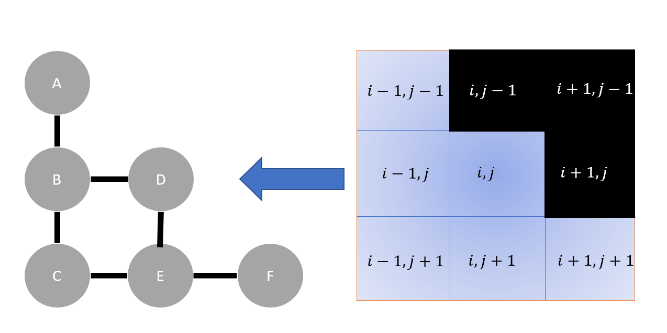
\includegraphics[width=0.8\linewidth]{figs/10/fig10_1}
	\caption{ تحويل فضاء العمل المقطع إلى بيان غير موجه}
	\label{fig:fig101}
\end{figure}

\subsubsection{المسار باستخدام A*}

خوارزمية عبور بيان وانشاء مسار تستخدم في كثير من مجالات علم الحاسوب نظرً لكمالها، مثاليتها، وكفاءتها. في الأنظمة التي من الممكن حساب الطريق بشكل استباقي، يمكن تجاوز أدائها من قبل الخوارزميات التي تستطيع حساب المسار قبل البدء بالتنفيذ \cite{d1} . واحدة من أكبر مشاكلها هي تعقيدها المكاني:$  O\left(b^d\right) $.

\subsubsection{المسار باستخدام Dijkstra}

هي خوارزمية صممت لإيجاد المسار الأقصر بين عقدتين في بيان معين. تعتمد الخوارزمية على إيجاد الطريق من خلال عبور عقد البيان بالتدريج ثم حساب معاملات المسافة وإيقاف البحث في حال مواجهة عائق \cite{d2}


\begin{table}
	\centering
	\begin{tabular}{cc}
		
		\begin{subfigure}{0.4\textwidth}
			\centering
			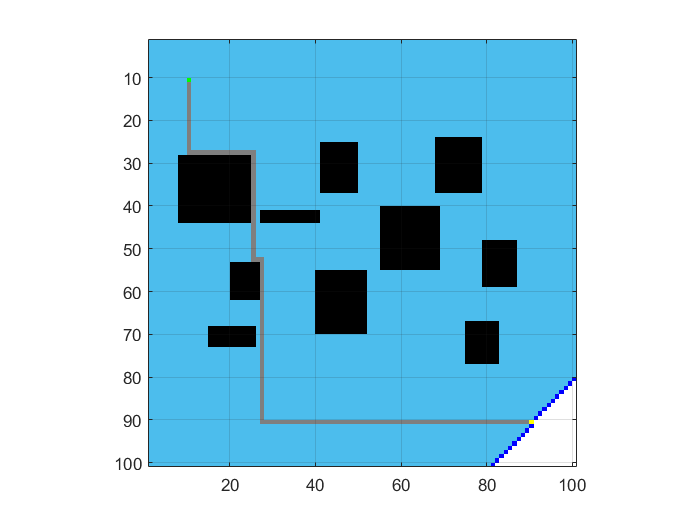
\includegraphics[width=0.9\linewidth]{figs/10/fig10_2}
		\end{subfigure}&
	
		\begin{subfigure}{0.4\textwidth}
			\centering
			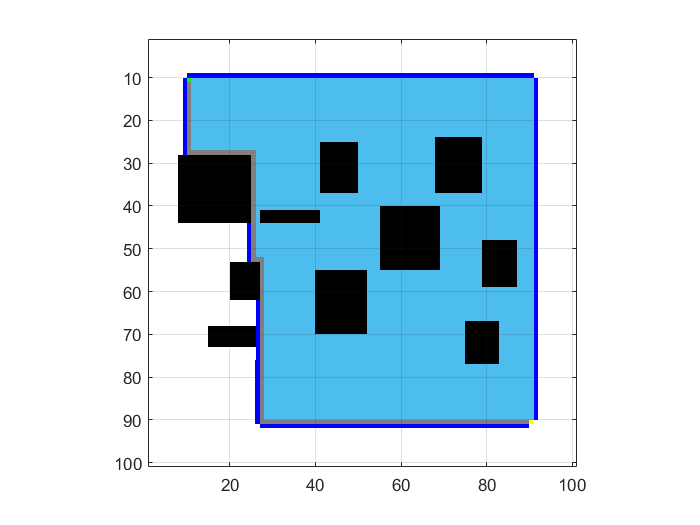
\includegraphics[width=0.9\linewidth]{figs/10/fig10_3}
		\end{subfigure}
	\end{tabular}
	\caption{خرائط لحل كل من خوارزميتي البيان.}
	\label{10:fig:graph}
\end{table}

\subsection{خوارزمية الحقل الكموني}
تعتمد خوارزمية \textenglish{potential field} على بناء خريطة افتراضية يتحرك الروبوت وفقها اعتماداً على مواقع المبدأ والهدف والحواجز. يمكن أن يتم حساب المسار اعتماداً على خريطة حواجز معروفة مسبقاً أو بالزمن الحقيقي اعتماداً على حساسات مثبتة على الروبوت أو على الحلبة. تم عرض هذه الخوارزمية لأول مرة عام 1985 \cite{b8} حيث قدم البحث الحقول $ potential field $ كجزئين، جزء جاذب وجزء منفر. الجزء الجاذب يقوم بسحب الروبوت نحو الهدف، أما الجزء المنفر يقوم بإبعاد الروبوت عن العوائق بمسافة أمان تحدد مسبقا. 

تستخدم هذه الخوارزمية بكثرة في تطبيقات تخطيط المسار وذلك لبساطتها وسهولة تطبيقها ولا سيما أنها تعطي نتائج جيدة في البيئات البسيطة التقليدية، لكن يوجد عدة سلبيات مرتبطة باستخدام هذه الخوارزمية.
أحد السلبيات هي أن الروبوت يمكن أن يحتجز في قيمة صغرى محلية مما يؤدي الى توقفه عن الحركة نهائيا وعدم وصوله الى الهدف. تم تطوير العديد من الطرق لحل هذه المشكلة متل تتبع الحائط   \cite{d4}  وإضافة حواجز افتراضية \cite{d5}. من السلبيات الأخرى هي عدم قدرة الروبوت على المرور بين حواجز متقاربة. عند عبور الروبوت بممر ضيق يقوم بحركة اهتزازية غير مستقرة نتيجة تأثره بقوى الحقل المنفر \cite{d6}.


\textbf{توليد المسار وفق $ potential field $:}

شعاع الحقل الجاذب يحسب من موقع الروبوت الى الهدف، أما شعاع الحقل المنفر يكون من موقع الحاجز الى موقع الروبوت. بجمع الشعاعين نحصل على شعاع يحدد اتجاهه اتجاه حركة الروبوت، ومطاله سرعة الروبوت. ليكن $ (x_r,y_r) $ موقع الربوت الابتدائي و $ (x_g,y_g) $ موقع الهدف و $ (x_o,\ y_o)   $ موقع الحاجز في خريطة ثنائية الأبعاد.

يعطى شعاع الحقل الجاذب بالعلاقات التالية:

\begin{equation}
{\vec{v}}_{attr}=\left(\begin{matrix}x_{atrr}\\y_{atrr}\\\end{matrix}  \right)
\end{equation}

\begin{equation}
\left(\begin{matrix}x_{atrr}\\y_{atrr}\\\end{matrix}  \right)=\left(\begin{matrix}x_{g} - x_{r}\\y_{g} - y{r}\\\end{matrix}  \right)
\end{equation}

تعطى المسافة والزاوية بين الروبوت والهدف بالعلاقات التالية:

\begin{equation}
d_o=\sqrt{\left(x_r-x_o\right)^2+\left(y_r-y_o\right)^2}
\end{equation}

\begin{equation}
\theta = tan^-1(\frac{y_r - y_o}{x_r - x_o})
\end{equation}

وبالتالي يعطى شعاع الحقل المنفر بالعلاقات التالية:

\begin{equation}
{\vec{v}}_{rep}=\ (\begin{matrix}x_{rep}\\y_{rep}\\\end{matrix})\ 
\end{equation}

\begin{equation}
x_{rep}=\frac{1}{d_o} cos(\theta), if d_o < s
x_red = 0 , otherwise  
\end{equation}

\begin{equation}
y_{rep}=\frac{1}{d_o} sin(\theta_o), if d_o < s
y_red = 0 , otherwise  
\end{equation}


حيث $ s $ هي قطر المنطقة الفعالية المحيطة بمركز الحاجز.
بجمع شعاعي الحركة الجاذب والمنفر نحصل على شعاع الحركة النهائي:

\begin{equation}
v_{final}^\rightarrow=v_{attr}^\rightarrow+v_{rep}^\rightarrow
\end{equation}

\begin{table}
	\centering
	\begin{tabular}{cc}
		
		\begin{subfigure}{0.35\textwidth}
			\centering
			\includesvg[width=0.9\linewidth]{figs/10/fig10_4}
		\end{subfigure}&
		
		\begin{subfigure}{0.35\textwidth}
			\centering
			\includesvg[width=0.9\linewidth]{figs/10/fig10_5}
		\end{subfigure}
	\end{tabular}
	\caption{عملية حساب المسار في طريقة الحقل الكموني}
	\label{10:fig:pf}
\end{table}


